\PassOptionsToPackage{unicode=true}{hyperref} % options for packages loaded elsewhere
\PassOptionsToPackage{hyphens}{url}
%
\documentclass[ignorenonframetext,]{beamer}
\usepackage{pgfpages}
\setbeamertemplate{caption}[numbered]
\setbeamertemplate{caption label separator}{: }
\setbeamercolor{caption name}{fg=normal text.fg}
\beamertemplatenavigationsymbolsempty
% Prevent slide breaks in the middle of a paragraph:
\widowpenalties 1 10000
\raggedbottom
\setbeamertemplate{part page}{
\centering
\begin{beamercolorbox}[sep=16pt,center]{part title}
  \usebeamerfont{part title}\insertpart\par
\end{beamercolorbox}
}
\setbeamertemplate{section page}{
\centering
\begin{beamercolorbox}[sep=12pt,center]{part title}
  \usebeamerfont{section title}\insertsection\par
\end{beamercolorbox}
}
\setbeamertemplate{subsection page}{
\centering
\begin{beamercolorbox}[sep=8pt,center]{part title}
  \usebeamerfont{subsection title}\insertsubsection\par
\end{beamercolorbox}
}
\AtBeginPart{
  \frame{\partpage}
}
\AtBeginSection{
  \ifbibliography
  \else
    \frame{\sectionpage}
  \fi
}
\AtBeginSubsection{
  \frame{\subsectionpage}
}
\usepackage{lmodern}
\usepackage{amssymb,amsmath}
\usepackage{ifxetex,ifluatex}
\usepackage{fixltx2e} % provides \textsubscript
\ifnum 0\ifxetex 1\fi\ifluatex 1\fi=0 % if pdftex
  \usepackage[T1]{fontenc}
  \usepackage[utf8]{inputenc}
  \DeclareUnicodeCharacter{03B5}{$\epsilon$}
  \DeclareUnicodeCharacter{03C3}{$\sigma$}
  \usepackage{textcomp} % provides euro and other symbols
\else % if luatex or xelatex
  \usepackage{unicode-math}
  \defaultfontfeatures{Ligatures=TeX,Scale=MatchLowercase}
\fi
% use upquote if available, for straight quotes in verbatim environments
\IfFileExists{upquote.sty}{\usepackage{upquote}}{}
% use microtype if available
\IfFileExists{microtype.sty}{%
\usepackage[]{microtype}
\UseMicrotypeSet[protrusion]{basicmath} % disable protrusion for tt fonts
}{}
\IfFileExists{parskip.sty}{%
\usepackage{parskip}
}{% else
\setlength{\parindent}{0pt}
\setlength{\parskip}{6pt plus 2pt minus 1pt}
}
\usepackage{hyperref}
\hypersetup{
            pdfborder={0 0 0},
            breaklinks=true}
\urlstyle{same}  % don't use monospace font for urls
\newif\ifbibliography
\usepackage{color}
\usepackage{fancyvrb}
\newcommand{\VerbBar}{|}
\newcommand{\VERB}{\Verb[commandchars=\\\{\}]}
\DefineVerbatimEnvironment{Highlighting}{Verbatim}{commandchars=\\\{\}}
% Add ',fontsize=\small' for more characters per line
\newenvironment{Shaded}{}{}
\newcommand{\AlertTok}[1]{\textcolor[rgb]{1.00,0.00,0.00}{\textbf{#1}}}
\newcommand{\AnnotationTok}[1]{\textcolor[rgb]{0.38,0.63,0.69}{\textbf{\textit{#1}}}}
\newcommand{\AttributeTok}[1]{\textcolor[rgb]{0.49,0.56,0.16}{#1}}
\newcommand{\BaseNTok}[1]{\textcolor[rgb]{0.25,0.63,0.44}{#1}}
\newcommand{\BuiltInTok}[1]{#1}
\newcommand{\CharTok}[1]{\textcolor[rgb]{0.25,0.44,0.63}{#1}}
\newcommand{\CommentTok}[1]{\textcolor[rgb]{0.38,0.63,0.69}{\textit{#1}}}
\newcommand{\CommentVarTok}[1]{\textcolor[rgb]{0.38,0.63,0.69}{\textbf{\textit{#1}}}}
\newcommand{\ConstantTok}[1]{\textcolor[rgb]{0.53,0.00,0.00}{#1}}
\newcommand{\ControlFlowTok}[1]{\textcolor[rgb]{0.00,0.44,0.13}{\textbf{#1}}}
\newcommand{\DataTypeTok}[1]{\textcolor[rgb]{0.56,0.13,0.00}{#1}}
\newcommand{\DecValTok}[1]{\textcolor[rgb]{0.25,0.63,0.44}{#1}}
\newcommand{\DocumentationTok}[1]{\textcolor[rgb]{0.73,0.13,0.13}{\textit{#1}}}
\newcommand{\ErrorTok}[1]{\textcolor[rgb]{1.00,0.00,0.00}{\textbf{#1}}}
\newcommand{\ExtensionTok}[1]{#1}
\newcommand{\FloatTok}[1]{\textcolor[rgb]{0.25,0.63,0.44}{#1}}
\newcommand{\FunctionTok}[1]{\textcolor[rgb]{0.02,0.16,0.49}{#1}}
\newcommand{\ImportTok}[1]{#1}
\newcommand{\InformationTok}[1]{\textcolor[rgb]{0.38,0.63,0.69}{\textbf{\textit{#1}}}}
\newcommand{\KeywordTok}[1]{\textcolor[rgb]{0.00,0.44,0.13}{\textbf{#1}}}
\newcommand{\NormalTok}[1]{#1}
\newcommand{\OperatorTok}[1]{\textcolor[rgb]{0.40,0.40,0.40}{#1}}
\newcommand{\OtherTok}[1]{\textcolor[rgb]{0.00,0.44,0.13}{#1}}
\newcommand{\PreprocessorTok}[1]{\textcolor[rgb]{0.74,0.48,0.00}{#1}}
\newcommand{\RegionMarkerTok}[1]{#1}
\newcommand{\SpecialCharTok}[1]{\textcolor[rgb]{0.25,0.44,0.63}{#1}}
\newcommand{\SpecialStringTok}[1]{\textcolor[rgb]{0.73,0.40,0.53}{#1}}
\newcommand{\StringTok}[1]{\textcolor[rgb]{0.25,0.44,0.63}{#1}}
\newcommand{\VariableTok}[1]{\textcolor[rgb]{0.10,0.09,0.49}{#1}}
\newcommand{\VerbatimStringTok}[1]{\textcolor[rgb]{0.25,0.44,0.63}{#1}}
\newcommand{\WarningTok}[1]{\textcolor[rgb]{0.38,0.63,0.69}{\textbf{\textit{#1}}}}
\usepackage{graphicx,grffile}
\makeatletter
\def\maxwidth{\ifdim\Gin@nat@width>\linewidth\linewidth\else\Gin@nat@width\fi}
\def\maxheight{\ifdim\Gin@nat@height>\textheight\textheight\else\Gin@nat@height\fi}
\makeatother
% Scale images if necessary, so that they will not overflow the page
% margins by default, and it is still possible to overwrite the defaults
% using explicit options in \includegraphics[width, height, ...]{}
\setkeys{Gin}{width=\maxwidth,height=\maxheight,keepaspectratio}
\setlength{\emergencystretch}{3em}  % prevent overfull lines
\providecommand{\tightlist}{%
  \setlength{\itemsep}{0pt}\setlength{\parskip}{0pt}}
\setcounter{secnumdepth}{0}

% set default figure placement to htbp
\makeatletter
\def\fps@figure{htbp}
\makeatother


\date{}

\begin{document}

\begin{frame}

\end{frame}

\begin{frame}{MuCoSim: MD-Bench on Cuda}
\protect\hypertarget{mucosim-md-bench-on-cuda}{}

{[}TOC{]}

\begin{block}{Project Description}

\begin{block}{Customer Info}

\begin{itemize}
\tightlist
\item
  Name: Martin Bauernfeind
\item
  E-Mail:
  \href{mailto:martin.m.bauernfeind@fau.de}{\nolinkurl{martin.m.bauernfeind@fau.de}}
\end{itemize}

\end{block}

\end{block}

\end{frame}

\begin{frame}

\begin{block}{Application Info}

\begin{itemize}
\tightlist
\item
  Code: MD-Bench on Cuda
\item
  URL:
  \href{https://github.com/RRZE-HPC/MD-Bench/tree/mucosim_cuda}{https://github.com/RRZE-HPC/MD-Bench/tree/mucosim\_cuda}
\end{itemize}

The original MD-Bench is a mini-app to simulate molecular dynamics. Its
code is written in sequential C with less than 1000 lines of code.
MD-Bench on Cuda is aimed to port this code to Cuda to use the power of
massive parallelism on GPGPUs. Even though many parts are already ported
to Cuda, significant parts still remain in C and therefore on the CPU.

*Note: The words particle and atom will be used interchangeably

\end{block}

\end{frame}

\begin{frame}

MD-Bench emulates such molecular dynamics by calculating the
interactions among particles and how these affect their motion. The
simulation system's constituents are

\begin{itemize}
\tightlist
\item
  Number of atoms with initial state (position \& velocity)
\item
  Boundary conditions (periodic)
\end{itemize}

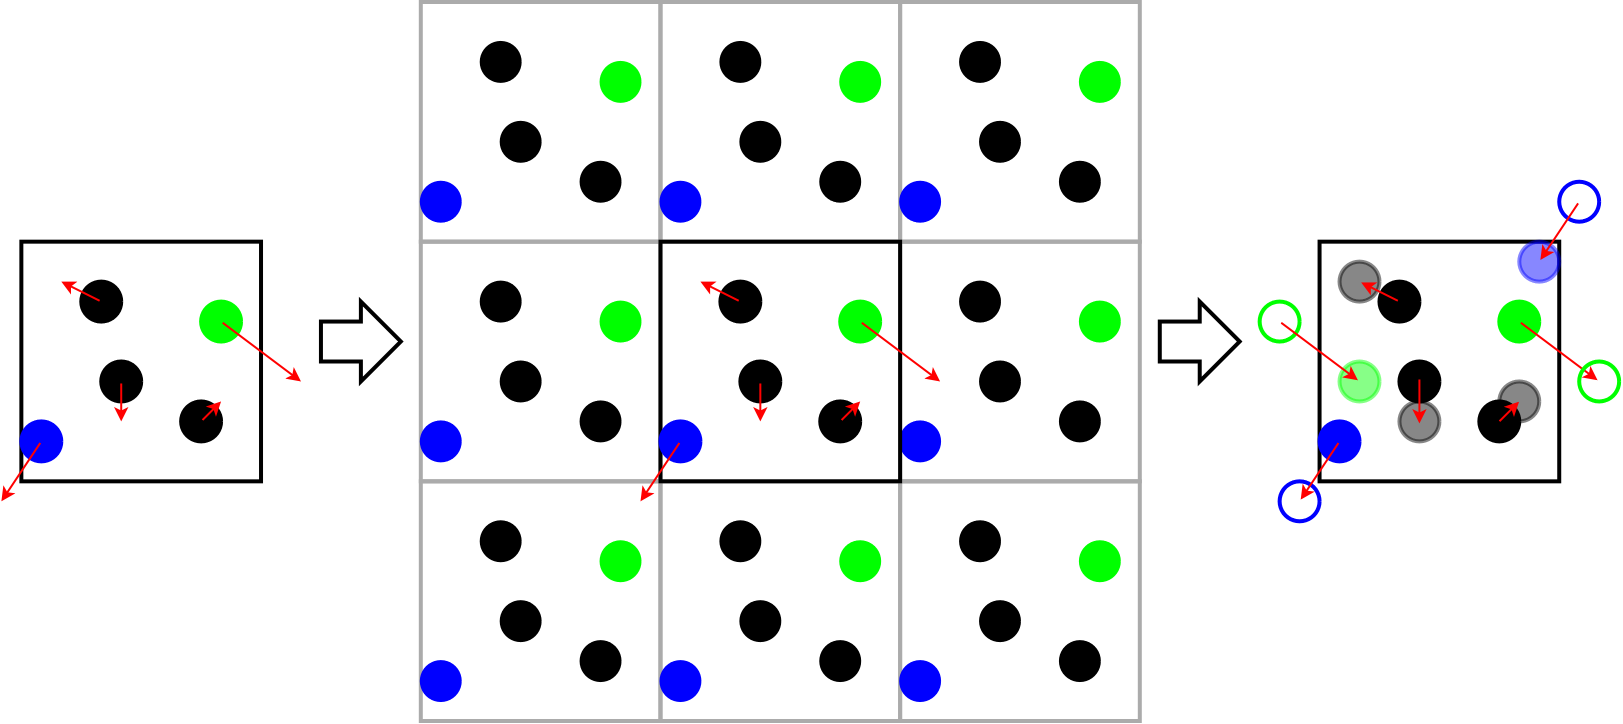
\includegraphics{../images/Boundary_Condition_explained_without_ghosts.png}

\end{frame}

\begin{frame}

force computation between atom:

\begin{itemize}
\tightlist
\item
  based on the Lennard-Jones potential:

  \begin{itemize}
  \tightlist
  \item
    pairs of particles, here: electronically neutral atoms
  \item
    models repulsive as well as attractive interactions
  \end{itemize}
\end{itemize}

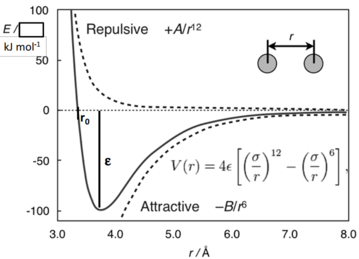
\includegraphics[width=0.5\textwidth]{../images/Lennard_Jones_potential_function.png}

\begin{itemize}
\tightlist
\item
  \emph{\textbf{r}} is the distance between the two interacting atoms,
\item
  \emph{\textbf{ε}} is the dispersion energy and
\item
  \emph{\textbf{σ}} the distance at which the particle-potential
  \emph{\textbf{V}} is zero
\end{itemize}

\end{frame}

\begin{frame}

What can be observed from this graph is:

\begin{itemize}
\tightlist
\item
  The Lennard-Jones potential is a simplified model but still describes
  the essential aspects of particle dynamics
\item
  Particles repel each other at close distances, attract each other at
  medium distances and have close to zero interaction at large distances
\end{itemize}

\end{frame}

\begin{frame}[fragile]

The simulation runs similar to the sketch code below:

\begin{itemize}
\tightlist
\item
  every timestep iterate over all particles:

  \begin{itemize}
  \tightlist
  \item
    compute interactions with neighbors
  \item
    integrate force generated by interaction
  \end{itemize}
\end{itemize}

\begin{scriptsize}
\begin{Shaded}
\begin{Highlighting}[]
\ControlFlowTok{for}\NormalTok{ t }\KeywordTok{in}\NormalTok{ timesteps:}
  \CommentTok{#GPU-parallel-for atom in atoms:}
\NormalTok{    velocity[atom] }\OperatorTok{+=}\NormalTok{ force[atom]}
\NormalTok{    position[atom] }\OperatorTok{+=}\NormalTok{ velocity[atom]}
  \ControlFlowTok{if}\NormalTok{ t }\OperatorTok{%} \DecValTok{20} \OperatorTok{==} \DecValTok{0}\NormalTok{:}
\NormalTok{    neighbors }\OperatorTok{=}\NormalTok{ calculateNeighbors()}
  \CommentTok{#GPU-parallel-for atom in atoms:}
\NormalTok{    neighbors }\OperatorTok{=}\NormalTok{ neighbors[atom]}
\NormalTok{    force }\OperatorTok{=} \FloatTok{0.0}
    \ControlFlowTok{for}\NormalTok{ neighbor }\KeywordTok{in}\NormalTok{ neighbors:}
\NormalTok{        radius }\OperatorTok{=}\NormalTok{ calc_radius(...)}
        \ControlFlowTok{if}\NormalTok{ radius }\OperatorTok{<}\NormalTok{ close_enough:}
\NormalTok{            force }\OperatorTok{+=}\NormalTok{ calc_force(...)}
\NormalTok{    forces[atom] }\OperatorTok{+=}\NormalTok{ force}
\end{Highlighting}
\end{Shaded}
\end{scriptsize}

Some parts already have been ported to GPU - more on that later

\end{frame}

\begin{frame}

\begin{block}{Testsystem}

\begin{itemize}
\tightlist
\item
  Host/Clustername: alex
\item
  Cluster Info URL:
  \href{https://hpc.fau.de/systems-services/systems-documentation-instructions/clusters/alex-cluster/}{https://hpc.fau.de/systems-services/systems-documentation-instructions/clusters/alex-cluster/}
\item
  per node:

  \begin{itemize}
  \tightlist
  \item
    CPU: 2x AMD EPYC 7713 ``Milan'' (64 cores per chip) @ 2.0 GHz - SMT
    disabled -\textgreater{} 1 Thread/CPU
  \item
    Memory capacity: {[}512 GB \textbar{} 1024 GB \textbar{} 512 GB{]}
  \item
    GPU: {[}8x A100/40GB \textbar{} 8x A100/80GB \textbar{} 8x
    A40/48GB{]}
  \end{itemize}
\item
  Info on single node jobs:
  \href{https://hpc.fau.de/systems-services/systems-documentation-instructions/clusters/alex-cluster/\#batch}{https://hpc.fau.de/systems-services/systems-documentation-instructions/clusters/alex-cluster/\#batch}
\item
  resources per GPU:

  \begin{itemize}
  \tightlist
  \item
    {[}A40 \textbar{} A100{]}
  \item
    CPU: {[}16 / GPU \textbar{} 16 / GPU{]}
  \item
    Memory: {[}60GB / GPU \textbar{} 120GB / GPU{]}
  \end{itemize}
\end{itemize}

\textbf{Note}: each an A40 has about double the single precision
processing power of an A100 despite being cheaper

\end{block}

\end{frame}

\begin{frame}[fragile]

\begin{block}{Software Environment}

\textbf{Compiler}:

\begin{itemize}
\tightlist
\item
  Compiler: NVCC (cuda/11.6.1)
\item
  Operating System: Ubuntu 20.04.3 LTS
\item
  Addition libraries:

  \begin{itemize}
  \tightlist
  \item
    LIKWID 5.2.0
  \end{itemize}
\end{itemize}

\end{block}

\begin{block}{How to build software}

\begin{verbatim}
$ git clone https://github.com/RRZE-HPC/MD-Bench/tree/mucosim_cuda
$ cd MD-Bench
$ module load likwid cuda
$ make
\end{verbatim}

\end{block}

\end{frame}

\begin{frame}[fragile]

\begin{block}{Testcase description}

If not stated otherwise these are the conditions for the simulation
benchmarking.

\begin{itemize}
\tightlist
\item
  the number of simulated atoms is 131072
\item
  floating numbers use double precision
\item
  force computation between atoms uses the lennard-jones model
\item
  one gpu with its associated cores are used for computation
\end{itemize}

\end{block}

\begin{block}{How to run software}

\begin{verbatim}
$ module load likwid cuda
$ cd MD-Bench
$ make
$ ./MDBench-NVCC
\end{verbatim}

\end{block}

\end{frame}

\begin{frame}[fragile]

\begin{block}{Initial: CPU Scaling runs}

\begin{itemize}
\tightlist
\item
  one gpu with its associated 16 cores is fixed
\item
  scale the number of CPU-Threads
\item
  output of our programm contains line displaying throughput in number
  of atom updates per second:
\end{itemize}

\begin{verbatim}
Performance: 7.18 million atom updates per second
\end{verbatim}

\end{block}

\end{frame}

\begin{frame}[fragile]

Now we plot the single- and double-precision performance for linearly
increasing numbers of \texttt{NUM\_THREADS} from 1 to 32:


\includegraphics{../resources/initial_testing/linear_cpu-threads_scaling/SingleGPU_cpu_scaling.png}

Similar convergence points in performance between the A40 and A100 hints
at bottlenecks independent of the gpu.

\end{frame}

\begin{frame}[fragile]

\begin{block}{Profiling the application}

In order to find such a bottleneck the runtime behaviour of the
application is monitored with the command line tool \texttt{nsys}:

\begin{verbatim}
srun nsys profile -o ./a40_profiling_run
\end{verbatim}

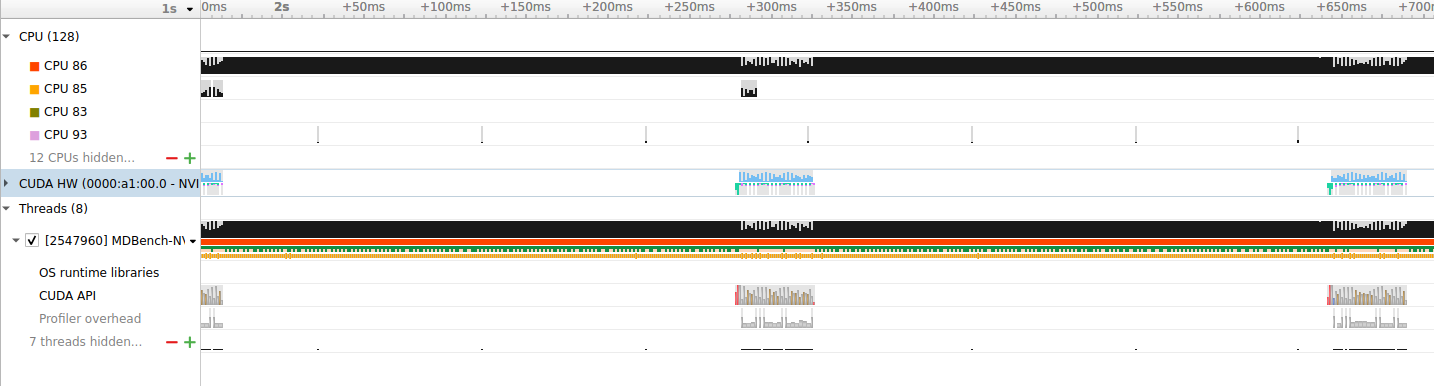
\includegraphics{../resources/initial_testing/finding_bottlenecks/using_nsys/A40_nsys_zoomed_in.png}

\begin{itemize}
\tightlist
\item
  activity is cyclic
\item
  most of the time is spent with only one CPU active
\item
  short blue parts are where the GPU is active
\end{itemize}

\end{block}

\end{frame}

\begin{frame}[fragile]

\begin{block}{Finding where the CPU time is spent}

Using the command line tool \texttt{gprof} we can see that most of the
CPU time is in the buildNeighbor-function

\begin{verbatim}
Flat profile:

Each sample counts as 0.01 seconds.
  %      self              total           
 time   seconds    calls  ms/call  name    
 97.70     3.35       11   306.47  buildNeighbor
  0.87     0.03      201     0.15  updatePbc
  0.58     0.02  2359296     0.00  myrandom
  0.58     0.02       11     1.82  binatoms
  0.29     0.01       11     0.91  setupPbc
  0.00     0.00     1668     0.00  checkCUDAError
  0.00     0.00      426     0.00  getTimeStamp
  0.00     0.00      201     0.00  computeForce
  0.00     0.00      200     0.00  cuda_final_integrate
  0.00     0.00      200     0.00  cuda_initial_integrate
...
\end{verbatim}

\end{block}

\end{frame}

\begin{frame}[fragile]

The standard program output also tells us in how much time (in total for
CPU and GPU) is used for neigbor selection and force computation. The
numbers will probably not match perfectly since gprof only samples the
CPU.

\begin{verbatim}
TOTAL 3.47s FORCE 0.21s NEIGH 3.15s REST 0.12s
\end{verbatim}

Even when considering CPU and GPU time the neighbor calculation needs
most of the time.

\end{frame}

\begin{frame}[fragile]

\begin{block}{Reasons for this runtime profile}

Recall code from earlier:

\begin{Shaded}
\begin{Highlighting}[]
\ControlFlowTok{for}\NormalTok{ t }\KeywordTok{in}\NormalTok{ timesteps:}
  \CommentTok{#GPU-parallel-for atom in atoms:}
\NormalTok{    velocity[atom] }\OperatorTok{+=}\NormalTok{ force[atom]}
\NormalTok{    position[atom] }\OperatorTok{+=}\NormalTok{ velocity[atom]}

  \ControlFlowTok{if}\NormalTok{ t }\OperatorTok{%} \DecValTok{20} \OperatorTok{==} \DecValTok{0}\NormalTok{:}
\NormalTok{    neighbors }\OperatorTok{=}\NormalTok{ calculate_neighbors()}

  \CommentTok{#GPU-parallel-for atom in atoms:}
\NormalTok{    neighbors }\OperatorTok{=}\NormalTok{ neighbors[atom]}
\NormalTok{    force }\OperatorTok{=} \FloatTok{0.0}
    \ControlFlowTok{for}\NormalTok{ neighbor }\KeywordTok{in}\NormalTok{ neighbors:}
\NormalTok{        radius }\OperatorTok{=}\NormalTok{ calc_radius(...)}
        \ControlFlowTok{if}\NormalTok{ radius }\OperatorTok{<}\NormalTok{ close_enough:}
\NormalTok{            force }\OperatorTok{+=}\NormalTok{ calc_force(...)}
\NormalTok{    forces[atom] }\OperatorTok{+=}\NormalTok{ force}
\end{Highlighting}
\end{Shaded}

\end{block}

\end{frame}

\begin{frame}[fragile]

\begin{block}{Parallelizing neighborhood calculation}

\begin{itemize}
\tightlist
\item
  real application simulates a 3D space
\item
  examples written in pseudo-python assume a 2D space
\end{itemize}

\begin{Shaded}
\begin{Highlighting}[]
\KeywordTok{def}\NormalTok{ calculate_neighbors():}
\NormalTok{  update_according_to(atoms, periodic_boundary_condition)}
\NormalTok{  setup_periodic_boundary_condition(atoms, periodic_boundary_condition)}
\NormalTok{  update_periodic_boundary_condition(atoms, periodic_boundary_condition)}
\NormalTok{  neighbor_list }\OperatorTok{=}\NormalTok{ build_neighbor(atoms)}
  \ControlFlowTok{return}\NormalTok{ neighbor_list}
\end{Highlighting}
\end{Shaded}

\end{block}

\end{frame}

\begin{frame}[fragile]

\begin{block}{Perodic boundary condition}

Atoms leaving the simulated area will enter on the mirrored side. In
code it looks like this:

\begin{Shaded}
\begin{Highlighting}[]
\KeywordTok{def}\NormalTok{ update_according_to(atoms, periodic_boundary_condition):}
\NormalTok{  sim_width, sim_height }\OperatorTok{=}\NormalTok{ periodic_boundary_condition.simulated_area.dims}
\NormalTok{  x_max, x_min, y_max, y_min }\OperatorTok{=}\NormalTok{ periodic_boundary_condition.boundaries}
  \ControlFlowTok{for}\NormalTok{ atom }\KeywordTok{in}\NormalTok{ atoms:}
    \ControlFlowTok{if}\NormalTok{ position[atom].x }\OperatorTok{>}\NormalTok{ x_max:}
\NormalTok{      position[atom].x }\OperatorTok{-=}\NormalTok{ sim_width}
    \ControlFlowTok{if}\NormalTok{ position[atom].x }\OperatorTok{<}\NormalTok{ x_min:}
\NormalTok{      position[atom].x }\OperatorTok{+=}\NormalTok{ sim_width}
    \ControlFlowTok{if}\NormalTok{ position[atom].y }\OperatorTok{>}\NormalTok{ y_max:}
\NormalTok{      position[atom].y }\OperatorTok{-=}\NormalTok{ sim_height}
    \ControlFlowTok{if}\NormalTok{ position[atom].y }\OperatorTok{<}\NormalTok{ y_min:}
\NormalTok{      position[atom].y }\OperatorTok{+=}\NormalTok{ sim_height}
\end{Highlighting}
\end{Shaded}

\begin{itemize}
\tightlist
\item
  all iterations indendent -\textgreater{} easy to parallelize
\item
  one thread per atom for simplicity (GPU threads are quite lightweight)
\end{itemize}

\end{block}

\end{frame}

\begin{frame}[fragile]

\begin{block}{Atoms near the periodic border}

Create ghost atoms on other side to emulate force interactions through
the periodic border

\begin{Shaded}
\begin{Highlighting}[]
\KeywordTok{def}\NormalTok{ setup_periodic_boundary_condition(atoms, periodic_boundary_condition):}
\NormalTok{  sim_width, sim_height }\OperatorTok{=}\NormalTok{ periodic_boundary_condition.simulated_area.dims}
\NormalTok{  x_max, x_min, y_max, y_min }\OperatorTok{=}\NormalTok{ periodic_boundary_condition.boundaries}
\NormalTok{  n_ghosts }\OperatorTok{=} \DecValTok{0}
\NormalTok{  n_ghost_allocations }\OperatorTok{=}\NormalTok{ some_value}
\NormalTok{  ghosts }\OperatorTok{=}\NormalTok{ malloc(n_ghost_allocations }\OperatorTok{*}\NormalTok{ sizeof(ghost))}
  
  \KeywordTok{def}\NormalTok{ createGhost(original_atom, offset_x, offset_y):}
\NormalTok{    ghost }\OperatorTok{=}\NormalTok{ \{\}}
\NormalTok{    ghost.original }\OperatorTok{=}\NormalTok{ original_atom}
\NormalTok{    ghost.offset_x }\OperatorTok{=}\NormalTok{ offset_x}
\NormalTok{    ghost.offset_y }\OperatorTok{=}\NormalTok{ offset_y}
    \ControlFlowTok{return}\NormalTok{ ghost}
  
  \ControlFlowTok{for}\NormalTok{ atom }\KeywordTok{in}\NormalTok{ atoms:}
    \ControlFlowTok{if}\NormalTok{ n_ghost_allocations }\OperatorTok{-}\NormalTok{ n_ghosts }\OperatorTok{<}\NormalTok{ max_ghosts_created_per_iteration:}
\NormalTok{      ghosts }\OperatorTok{=}\NormalTok{ realloc(ghosts, n_ghost_allocations, n_ghost_allocations }\OperatorTok{+}\NormalTok{ some_more)}
\NormalTok{      n_ghost_allocations }\OperatorTok{+=}\NormalTok{ some_more}
    \ControlFlowTok{if}\NormalTok{ position[atom].x }\OperatorTok{>}\NormalTok{ x_max }\OperatorTok{-}\NormalTok{ threshold:}
\NormalTok{      ghosts[n_ghosts}\OperatorTok{++}\NormalTok{] }\OperatorTok{=}\NormalTok{ createGhost(atom, }\OperatorTok{-}\NormalTok{sim_width, }\DecValTok{0}\NormalTok{)}
    \ControlFlowTok{if}\NormalTok{ position[atom].x }\OperatorTok{<}\NormalTok{ x_min }\OperatorTok{+}\NormalTok{ threshold:}
\NormalTok{      ghosts[n_ghosts}\OperatorTok{++}\NormalTok{] }\OperatorTok{=}\NormalTok{ createGhost(atom, }\OperatorTok{+}\NormalTok{sim_width, }\DecValTok{0}\NormalTok{)}
    \ControlFlowTok{if}\NormalTok{ position[atom].y }\OperatorTok{>}\NormalTok{ y_max }\OperatorTok{-}\NormalTok{ threshold:}
\NormalTok{      ghosts[n_ghosts}\OperatorTok{++}\NormalTok{] }\OperatorTok{=}\NormalTok{ createGhost(atom, }\DecValTok{0}\NormalTok{, }\OperatorTok{-}\NormalTok{sim_height)}
\NormalTok{    ...}
    \ControlFlowTok{if}\NormalTok{ position[atom].x }\OperatorTok{<}\NormalTok{ x_min }\OperatorTok{+}\NormalTok{ threshold AND position[atom] }\OperatorTok{<}\NormalTok{ y_min }\OperatorTok{+}\NormalTok{ threshold:}
\NormalTok{      ghosts[n_ghosts}\OperatorTok{++}\NormalTok{] }\OperatorTok{=}\NormalTok{ createGhost(atom, }\OperatorTok{+}\NormalTok{sim_width, }\OperatorTok{+}\NormalTok{sim_height)}
  
  \ControlFlowTok{if}\NormalTok{ n_atoms }\OperatorTok{+}\NormalTok{ n_ghosts }\OperatorTok{>} \BuiltInTok{len}\NormalTok{(atoms):}
\NormalTok{    atoms }\OperatorTok{=}\NormalTok{ realloc(n_atoms }\OperatorTok{+}\NormalTok{ n_ghosts)}
\end{Highlighting}
\end{Shaded}

\begin{itemize}
\tightlist
\item
  iterations depend on each other via the n\_ghosts variable
  -\textgreater{} parallelizing will be difficult
\end{itemize}

Ideas to parallelize: allocate more space for ghosts than will be needed
and give each atom a thread

\begin{itemize}
\tightlist
\item
  each thread inserts its atoms ghosts into a predefined empty space

  \begin{itemize}
  \tightlist
  \item
    -\textgreater{} no collisions but array will be sparsely occupied
  \end{itemize}
\item
  each thread atomically increments a global counter (mimicing the
  nghosts variable)

  \begin{itemize}
  \tightlist
  \item
    -\textgreater{} no collisions and dense array occupation, but
    atomicAdd might lead to lots of blocking
  \end{itemize}
\end{itemize}

\end{block}

\end{frame}

\begin{frame}[fragile]

\begin{block}{Updating the ghost atom positions}

\begin{Shaded}
\begin{Highlighting}[]
\KeywordTok{def}\NormalTok{ update_bondary_condition(atoms, periodic_boundary_condition):}
  \ControlFlowTok{for}\NormalTok{ ghost }\KeywordTok{in}\NormalTok{ ghosts:}
\NormalTok{    position[ghost].x }\OperatorTok{=}\NormalTok{ ghost.offset_x }\OperatorTok{+}\NormalTok{ position[ghost.original].x}
\NormalTok{    position[ghost].y }\OperatorTok{=}\NormalTok{ ghost.offset_y }\OperatorTok{+}\NormalTok{ position[ghost.original].y}
\end{Highlighting}
\end{Shaded}

\begin{itemize}
\tightlist
\item
  iterations independent

  \begin{itemize}
  \tightlist
  \item
    -\textgreater{} easy to parallelize
  \item
    -\textgreater{} one thread per atom
  \end{itemize}
\end{itemize}

\end{block}

\begin{block}{Building neighbor lists}

\begin{itemize}
\tightlist
\item
  majority of time is spent here

  \begin{itemize}
  \tightlist
  \item
    parallelizing will probably reduce runtime sigificantly
  \end{itemize}
\end{itemize}

\begin{Shaded}
\begin{Highlighting}[]
\KeywordTok{def}\NormalTok{ buildNeighbor(atoms):}
\NormalTok{  max_neighbors_per_atom }\OperatorTok{=}\NormalTok{ some_value}
\NormalTok{  new_max_neighbors_per_atom }\OperatorTok{=}\NormalTok{ max_neighbors_per_atom}
\NormalTok{  grid_cells }\OperatorTok{=}\NormalTok{ sort_into(atoms)}
\NormalTok{  neighbor_list }\OperatorTok{=}\NormalTok{ malloc(n_atoms }\OperatorTok{*}\NormalTok{ max_neighbors }\OperatorTok{*}\NormalTok{ sizeof(}\BuiltInTok{int}\NormalTok{))}
\NormalTok{  neighbor_counters }\OperatorTok{=}\NormalTok{ malloc(n_atoms }\OperatorTok{*}\NormalTok{ sizeof(}\BuiltInTok{int}\NormalTok{))}
  
\NormalTok{  resize_needed }\OperatorTok{=}\NormalTok{ true}
  \ControlFlowTok{while}\NormalTok{(resize_needed):}
\NormalTok{    new_max_neighbors_per_atom }\OperatorTok{=}\NormalTok{ max_neighbors_per_atom}
\NormalTok{    resize_needed }\OperatorTok{=}\NormalTok{ false}
    \ControlFlowTok{for}\NormalTok{ atom }\KeywordTok{in}\NormalTok{ atoms:}
\NormalTok{      neighbor_count }\OperatorTok{=} \DecValTok{0}
\NormalTok{      grid_cell }\OperatorTok{=}\NormalTok{ grid_cell_of(position[atom])}
      \ControlFlowTok{for}\NormalTok{ neighboring_cell }\KeywordTok{in}\NormalTok{ neighboring_cells(grid_cell):}
        \ControlFlowTok{for}\NormalTok{ possible_neighbor }\KeywordTok{in}\NormalTok{ neighboring_cell.atoms:}
          \ControlFlowTok{if}\NormalTok{ distance(atom, possible_neighbor) }\OperatorTok{<}\NormalTok{ threshold:}
\NormalTok{            neighbor_list[atom }\OperatorTok{*}\NormalTok{ max_neighbors_per_atom }\OperatorTok{+}\NormalTok{ neighbor_count] }\OperatorTok{=}\NormalTok{ possible_neighbor}
\NormalTok{            neighbor_count}\OperatorTok{++}
      \ControlFlowTok{if}\NormalTok{ neighbor_count }\OperatorTok{>}\NormalTok{ max_neighbors_per_atom:}
\NormalTok{        resize_needed }\OperatorTok{=}\NormalTok{ true}
        \ControlFlowTok{if}\NormalTok{ neighbor_count }\OperatorTok{>}\NormalTok{ new_max_neighbor_count_per_atom:}
\NormalTok{          new_max_neighbor_count_per_atom }\OperatorTok{=}\NormalTok{ neighbor_count}
    \ControlFlowTok{if}\NormalTok{ resize_needed:}
\NormalTok{      max_neighbors_per_atom }\OperatorTok{=}\NormalTok{ new_max_neighbors_per_atom }\OperatorTok{*} \FloatTok{1.2}
\NormalTok{      free(neighbor_list)}
\NormalTok{      neihgbor_list }\OperatorTok{=}\NormalTok{ malloc(n_atoms }\OperatorTok{*}\NormalTok{ max_neighbors }\OperatorTok{*}\NormalTok{ sizeof(}\BuiltInTok{int}\NormalTok{))}
\end{Highlighting}
\end{Shaded}

\begin{itemize}
\tightlist
\item
  iterations over atoms are output dependent on each other iff neighbor
  lists are longer than the individually allocated space
\end{itemize}

\end{block}

\begin{block}{Next goals}

ordered by priority

\begin{itemize}
\item
  port the buildNeighbor-function to Cuda (reduced Host-To-Device
  traffic, reduced computation time)
\item
  port the function updating the ghost atoms to Cuda
\item
  port the creating the ghost atoms to Cuda
\item
  evaluate performance along the way
\end{itemize}

\end{block}

\end{frame}

\end{document}
